% RTKLIB source file
\section{RTKLIB源程序}
\begin{frame}{单点定位RTCM}
    \begin{itemize}
        \item RTCM file
        \begin{figure}
            \centering
            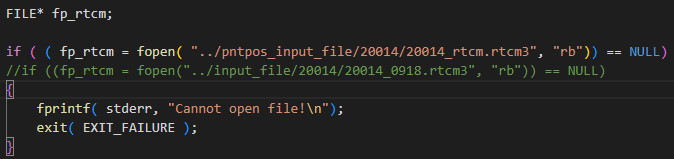
\includegraphics[width=.5\textwidth]{pic/rtcm_file.png}
            \caption{RTCM文件}
            \label{fig:rtcm_file}
        \end{figure}
        \item 单点定位配置
        \begin{figure}
            \centering
            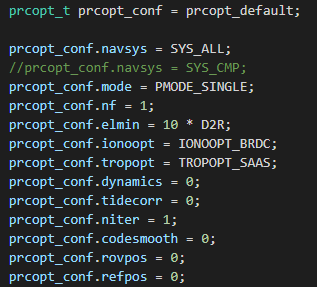
\includegraphics[width=.3\textwidth]{pic/prcopt_config.png}
            \caption{单点定位配置}
            \label{fig:pnt_config}
        \end{figure}
    \end{itemize}
\end{frame}

\begin{frame}{nav数据结构初始化声明}
    \begin{figure}
        \centering
        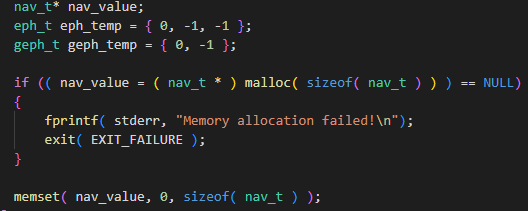
\includegraphics[width=.5\textwidth]{pic/nav_data_memset.png}
        \caption{nav数据}
        \label{fig:nav_data}
    \end{figure}
\end{frame}

\begin{frame}{求解流程}
    \begin{figure}
        \centering
        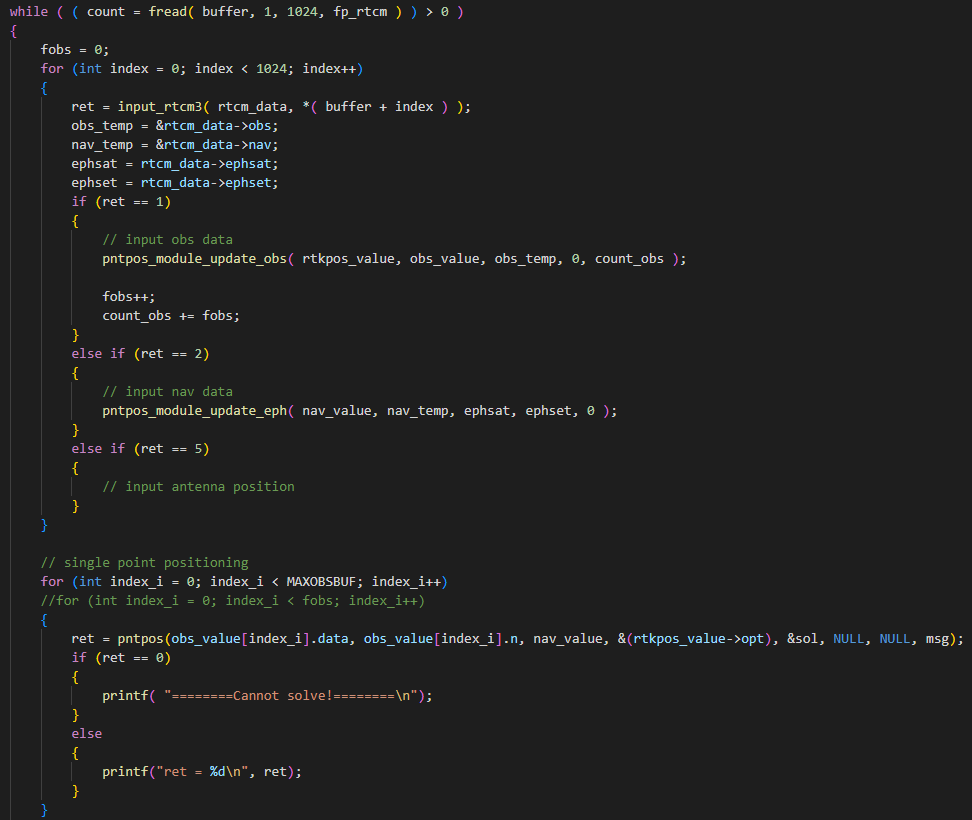
\includegraphics[width=.5\textwidth]{pic/pntpos_process.png}
        \caption{逻辑流程}
        \label{fig:pntpos_process}
    \end{figure}
\end{frame}

\section{Future work}
\begin{frame}{Future}
    \begin{itemize}
        \item LAMBDA算法文献调研
        \item 离散型优化算法
        \item 网平差算法
        \item 国产化平台JAVA调用C程序.so文件打包
    \end{itemize}
\end{frame}